\chapter{Transformações Lineares}
Neste capítulo, iremos tratar sobre um tipo especial de função ou aplicação, onde, segundo \cite{steinbruch1987}, o domínio e o contradomínio são espaços vetoriais reais. Assim, tanto a variável independente como a variável dependente são vetores, razão pela qual essas funções são chamadas vetoriais.

Nosso estudo das funções vetoriais lineares em questão, será focado, nas transformações lineares.

\noindent\textbf{Definição 04:} Sejam V e W dois espaços vetoriais. Uma transformação linear (aplicação linear) é uma função de V em W, $F:V \rightarrow W$, que satisfaz as seguintes condições:
\begin{enumerate}
	\item Para quaisquer $u$ e $v$ em $V$, $F(u + v) = F(u) + F(v)$.
	\item Para quaisquer $k \in \mathbb{R}$ e $v \in V$, $F(kv) = kF(v)$.
\end{enumerate}	
\noindent\centerline{$\forall\mathbf{v}, \mathbf{v} \in \mathbf{V}$ e $\forall k \in \mathbb{R}$.}
Para se dizer que $\mathbf{T}$ é uma transformação linear do espaço vetorial $\mathbf{V}$ no espaço vetorial $\mathbf{W}$, será denotado por $\mathbf{T}:\mathbf{V}\longrightarrow\mathbf{W}$, onde $\mathbf{T}$ é a função, cada vetor $\mathbf{v} \in \mathbf{V}$ tem uma só imagem $\mathbf{w} \in \mathbf{W}$, indicado por $\mathbf{w} = \mathbf{T}(\mathbf{v})$.

Tomemos por dois conjuntos de vetores, $\mathbf{V} = \mathbb{R}^2$ e $\mathbf{W} = \mathbb{R}^3$.

Uma transformação de $\mathbf{T}:\mathbb{R}^2\longrightarrow\ \mathbb{R}^3$ associa vetores $\mathbf{v} = (x, y) \in \mathbb{R}^2$ com vetores $\mathbf{w} = (x, y, z) \in \mathbb{R}^3$

\noindent\textbf{Exemplo 11:} Declarado esta transformação linear $\mathbf{T}(x, y) = (x, y, x + y)$. Iremos selecionar alguns vetores em $\mathbb{R}^2$ e calcular suas imagens sob a transformação $\mathbf{T}$. Por exemplo, os vetores $(1, 0)$ e $(0, 1)$. Para $(1, 0)$, temos: 

\centerline{$\mathbf{T}(1, 0) = (1, 0, 1 +0) = (1, 0, 1)$}

\noindent e para $(0, 1)$, temos:

\centerline{$\mathbf{T}(0, 1) = (0, 1, 0 + 1) = (0, 1, 1)$.}

Segue a imagem em $\mathbb{R}^3$:

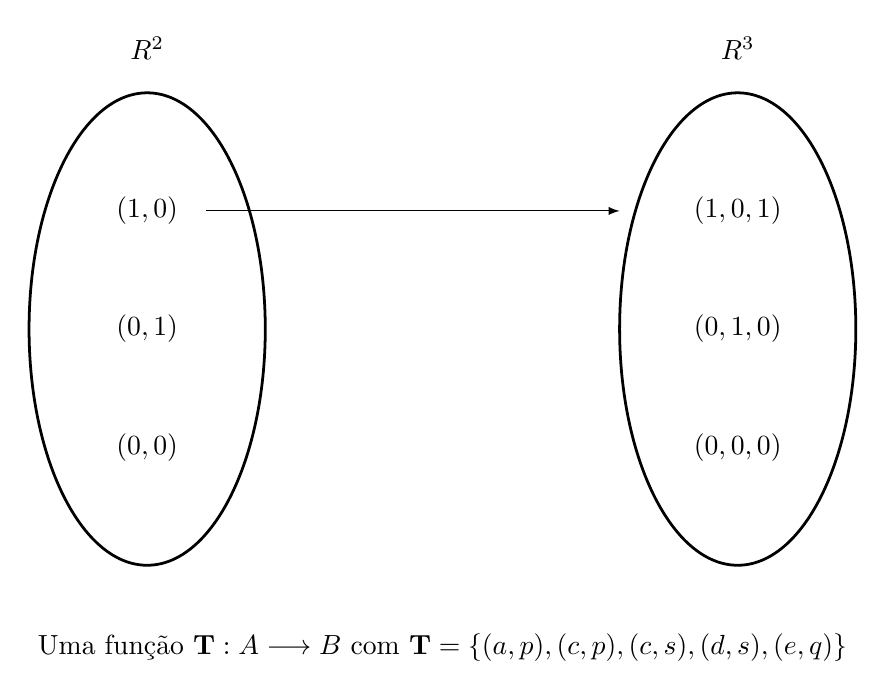
\begin{tikzpicture}[scale=1.5]
	\centering
	% Set A
	\draw[line width=1pt] (0,0) ellipse (1cm and 2cm);
	\node[above] at (0,2.2) (A) {$\mathbb{R}^2$};
	\node[centered] at (0,1) {$(1,0)$};
	\node[centered] at (0,0) {$(0,1)$};
	\node[centered] at (0,-1) {$(0,0)$};
	% Set B
	\draw[line width=1pt] (5,0) ellipse (1cm and 2cm);
	\node[above] at (5,2.2) (B) {$\mathbb{R}^3$};
	\node[centered] at (5,1) {$(1,0,1)$}; 
	\node[centered] at (5,0) {$(0,1,0)$};
	\node[centered] at (5,-1) {$(0,0,0)$};
	
	% Relations
	\draw[-latex, black] (0.5,1) -- (4,1);
	%\draw[-latex,cyan] (a) -- (p);
	%\draw[-latex,cyan] (c) -- (p);
	%\draw[-latex,cyan] (d) -- (s);
	%\draw[-latex,cyan] (e) -- (q);
	
	% Label
	\node[below] at (2.5,-2.5) {Uma função $\mathbf{T}: A \longrightarrow B$ com $\mathbf{T}=\{(a,p),(c,p),(c,s),(d,s),(e,q)\}$};
\end{tikzpicture}
	
